\documentclass[a4paper,11pt]{article}

\usepackage{amsmath}
\usepackage{tikz}
\usetikzlibrary{arrows,automata,shapes}

\newtheorem{theorem}{Theorem}
\newtheorem{corollary}{Corollary}[theorem]
\newtheorem{lemma}[theorem]{Lemma}

\begin{document}

\title{On Bulks and Sculptures}

\author{Christopher A. Trotter}

\maketitle

When talking about sculptures and bulks, Uli and I seem to agree that a 3x2 2-grid is a sculpture. Following the notation given by Uli, we can see that there is a way to labeling the squares such that all squares have a unique labeling. Given the example below, one can see that this is a sculpture.

\begin{lemma}
    The 3x2 2-grid is a sculpture.
\end{lemma}

\noindent PROOF (SKETCH) We start by labeling the squares as so (the number of 0s
at the end is unimportant; this works in any dimension):

\begin{center}
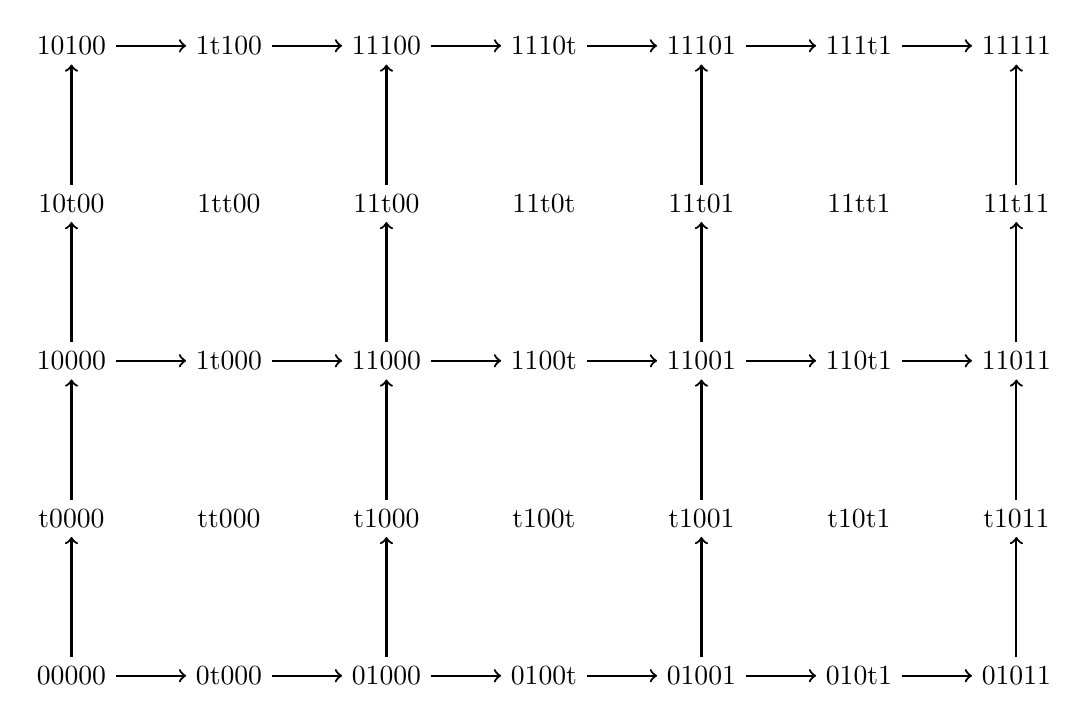
\begin{tikzpicture}[node distance=2cm, align=center]
    \title{3x2 2-grid Sculpture}
    % square 1
    \node(00000)                    {00000};
    \node(0t000) [right of=00000]   {0t000};
    \node(t0000) [above of=00000]   {t0000};
    \node(01000) [right of=0t000]   {01000};
    \node(10000) [above of=t0000]   {10000};
    \node(tt000) [right of=t0000]   {tt000};
    \node(t1000) [right of=tt000]   {t1000};
    \node(1t000) [right of=10000]   {1t000};
    \node(11000) [right of=1t000]   {11000};
    
    %square 2
    \node(10t00) [above of=10000]   {10t00};
    \node(10100) [above of=10t00]   {10100};
    \node(1tt00) [right of=10t00]   {1tt00};
    \node(11t00) [right of=1tt00]   {11t00};
    \node(1t100) [right of=10100]   {1t100};
    \node(11100) [right of=1t100]   {11100};
    
    %square 3
    \node(0100t) [right of=01000]   {0100t};
    \node(01001) [right of=0100t]   {01001};
    \node(t100t) [above of=0100t]   {t100t};
    \node(1100t) [above of=t100t]   {1100t};
    \node(t1001) [above of=01001]   {t1001};
    \node(11001) [above of=t1001]   {11001};
    
    %square 4
    \node(010t1) [right of=01001]   {010t1};
    \node(01011) [right of=010t1]   {01011};
    \node(t1011) [above of=01011]   {t1011};
    \node(11011) [above of=t1011]   {11011};
    \node(t10t1) [above of=010t1]   {t10t1};
    \node(110t1) [above of=t10t1]   {110t1};
    
    %square 5
    \node(11t0t) [above of=1100t]   {11t0t};
    \node(1110t) [above of=11t0t]   {1110t};
    \node(11t01) [above of=11001]   {11t01};
    \node(11101) [above of=11t01]   {11101};

    %square 6
    \node(11t11) [above of=11011]   {11t11};
    \node(11111) [above of=11t11]   {11111};
    \node(11tt1) [above of=110t1]   {11tt1};
    \node(111t1) [above of=11tt1]   {111t1};
    
    %square 1
    \draw [->][draw=black, thick] (00000) to node [below] {} (0t000);
    \draw [->][draw=black, thick] (00000) to node [left] {} (t0000);
    \draw [->][draw=black, thick] (0t000) to node [below] {} (01000);
    \draw [->][draw=black, thick] (t0000) to node [left] {} (10000);
    \draw [->][draw=black, thick] (10000) to node [left] {} (1t000);
    \draw [->][draw=black, thick] (1t000) to node [left] {} (11000);
    \draw [->][draw=black, thick] (01000) to node [left] {} (t1000);
    \draw [->][draw=black, thick] (t1000) to node [left] {} (11000);
    
    %square 2
    \draw [->][draw=black, thick] (10000) to node [below] {} (10t00);
    \draw [->][draw=black, thick] (10t00) to node [below] {} (10100);
    \draw [->][draw=black, thick] (11000) to node [below] {} (11t00);
    \draw [->][draw=black, thick] (11t00) to node [below] {} (11100);
    \draw [->][draw=black, thick] (10100) to node [below] {} (1t100);
    \draw [->][draw=black, thick] (1t100) to node [below] {} (11100);
    
    %square 3
    \draw [->][draw=black, thick] (01000) to node [below] {} (0100t);
    \draw [->][draw=black, thick] (0100t) to node [below] {} (01001);
    \draw [->][draw=black, thick] (01001) to node [below] {} (t1001);
    \draw [->][draw=black, thick] (t1001) to node [below] {} (11001);
    \draw [->][draw=black, thick] (1100t) to node [below] {} (11001);
    \draw [->][draw=black, thick] (11000) to node [below] {} (1100t);
    
    %square 4
    \draw [->][draw=black, thick] (01001) to node [below] {} (010t1);
    \draw [->][draw=black, thick] (010t1) to node [below] {} (01011);
    \draw [->][draw=black, thick] (01011) to node [below] {} (t1011);
    \draw [->][draw=black, thick] (t1011) to node [below] {} (11011);
    \draw [->][draw=black, thick] (110t1) to node [below] {} (11011);
    \draw [->][draw=black, thick] (11001) to node [below] {} (110t1);
    
    %square 5
    \draw [->][draw=black, thick] (11100) to node [below] {} (1110t);
    \draw [->][draw=black, thick] (1110t) to node [below] {} (11101);
    \draw [->][draw=black, thick] (11001) to node [below] {} (11t01);
    \draw [->][draw=black, thick] (11t01) to node [below] {} (11101);
    
    %square 6
    \draw [->][draw=black, thick] (11101) to node [below] {} (111t1);
    \draw [->][draw=black, thick] (111t1) to node [below] {} (11111);
    \draw [->][draw=black, thick] (11t11) to node [below] {} (11111);
    \draw [->][draw=black, thick] (11011) to node [below] {} (11t11);
  \end{tikzpicture}
 \end{center}
 
 It is possible to generate the 3x2 2-grid above, by consistently following the convention that:

\begin{itemize}
    \item A step can only move up or to the right.
    \item A '0' can be replaced by a 't'.
    \item If a step is made in the same direction, after adding a 't', then the 't' in this step is replaced by a '1'.
    \item Each middle square is a combination by the left and bottom edge. For example, the square '11t0t' is the combination of '11t00' and '1100t'.
    \item Lastly, each label must be unique.
\end{itemize}

\noindent \textbf{Note:} In the notes Uli provided, one can see that the proof sketch provided is such that it considered only up to 4th dimension. The same situation will occur even with a 2x2 2-grid.

\begin{lemma}
    The 2x2 2-grid is not a sculpture if the neighboring tiles, left and bottom, of the upper-right tile have to place a 't' on the same index of the upper-right tile.
\end{lemma}

\noindent PROOF (SKETCH) We start by labeling the squares as so (the number of 0s
at the end is unimportant; this works in any dimension):

\begin{center}
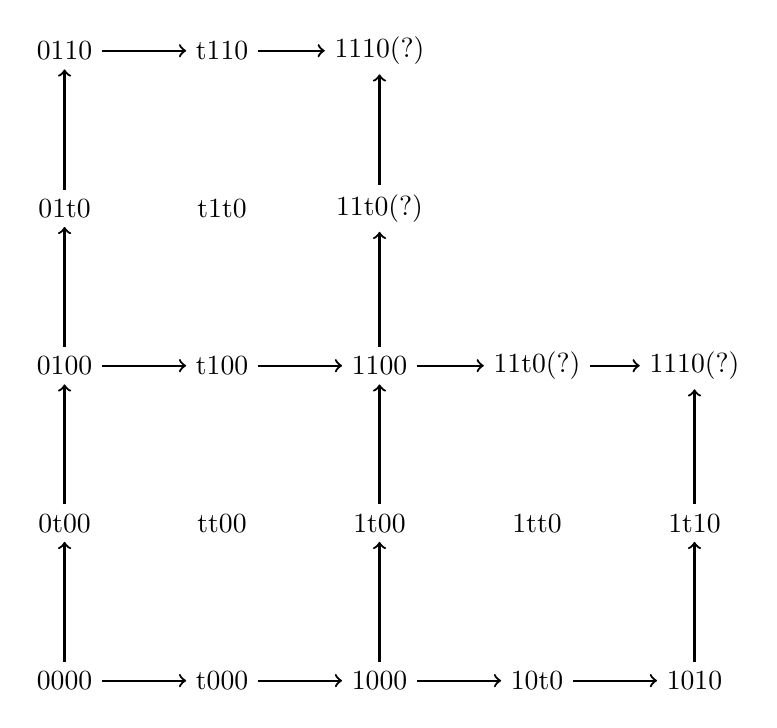
\begin{tikzpicture}[node distance=2cm, align=center]
    \title{unfolded HDA}
    
    % square 1
    \node(0000)                     {0000};
    \node(t000) [right of=0000]     {t000};
    \node(1000) [right of=t000]     {1000};
    \node(0t00) [above of=0000]     {0t00};
    \node(0100) [above of=0t00]     {0100};
    \node(tt00) [above of=t000]     {tt00};
    \node(1t00) [above of=1000]     {1t00};
    \node(t100) [above of=tt00]     {t100};
    \node(1100) [above of=1t00]     {1100};
    
    %square 2
    \node(10t0) [right of=1000]     {10t0};
    \node(1010) [right of=10t0]     {1010};
    \node(1tt0) [above of=10t0]     {1tt0};
    \node(1t10) [above of=1010]     {1t10};
    \node(11t0x) [above of=1tt0]     {11t0(?)};
    \node(1110x) [above of=1t10]     {1110(?)};
    
    %square 3
    \node(01t0) [above of=0100]     {01t0};
    \node(0110) [above of=01t0]     {0110};
    \node(t1t0) [above of=t100]     {t1t0};
    \node(11t0) [above of=1100]     {11t0(?)};
    \node(t110) [above of=t1t0]     {t110};
    \node(1110) [above of=11t0]     {1110(?)};
    
    
    %square 1
    \draw [->][draw=black, thick] (0000) to node [below] {} (t000);
    \draw [->][draw=black, thick] (0000) to node [left] {} (0t00);
    \draw [->][draw=black, thick] (t000) to node [left] {} (1000);
    \draw [->][draw=black, thick] (0t00) to node [left] {} (0100);
    \draw [->][draw=black, thick] (1000) to node [left] {} (1t00);
    \draw [->][draw=black, thick] (1t00) to node [left] {} (1100);
    \draw [->][draw=black, thick] (0100) to node [left] {} (t100);
    \draw [->][draw=black, thick] (t100) to node [left] {} (1100);
    
    %square 2
    \draw [->][draw=black, thick] (1000) to node [left] {} (10t0);
    \draw [->][draw=black, thick] (10t0) to node [left] {} (1010);
    \draw [->][draw=black, thick] (1010) to node [left] {} (1t10);
    \draw [->][draw=black, thick] (1t10) to node [left] {} (1110x);
    \draw [->][draw=black, thick] (1100) to node [left] {} (11t0x);
    \draw [->][draw=black, thick] (11t0x) to node [left] {} (1110x);
    
    %square 3
    \draw [->][draw=black, thick] (0100) to node [left] {} (01t0);
    \draw [->][draw=black, thick] (01t0) to node [left] {} (0110);
    \draw [->][draw=black, thick] (0110) to node [left] {} (t110);
    \draw [->][draw=black, thick] (t110) to node [left] {} (1110);
    \draw [->][draw=black, thick] (1100) to node [left] {} (11t0);
    \draw [->][draw=black, thick] (11t0) to node [left] {} (1110);

  \end{tikzpicture}
 \end{center}

\noindent By assuming the first argument provided in the notes:
\begin{itemize}
    \item 1tt0 and t1t0 are the only possible neighbors of tt00.
\end{itemize}

Note that we don't have much choice for the labeling.

\noindent Then we have the situation, as shown in the figure above, and it directly follows by the proof in the notes.

\end{document}